%!TEX root = ../main.tex
\documentclass[../main]{subfiles}
\begin{document}
  \chapter{Method}\label{chapter:method}

  In this chapter we review the current methods for numerically solving partial-integro differential equations. We begin by considering the simplest model for the Advection Equation, which serves as a model for the McKendrick-von Foerster Equation with constant coefficients. We will discuss the boundary conditions and domain, before adding in the diffusion term. Finally we consider the work of \cite{hartvig2011} who discusses a stable first order method for the McKendrick-von Foerster Equation when integral coefficients are used.

  \section{Upwind / Downwind Scheme}
  \begin{equation}
    L(u) = \frac{\partial u}{\partial t} + g \frac{\partial u}{\partial x} - \mu \cdot u
  \end{equation}

  We consider for the advection equation with the source term on the domain $[0, T] \times [0, X]$. By simply replacing the time derivative with a forward difference, and the spatial derivative with a backwards difference we can get a first order approximation

  which gives a finite difference equation

  \begin{equation}
    D(u) = \frac{u^{n+1}_j - u^n}{h} + g \frac{u^n_{j} - u^n_{j-1}}{k} - \mu u^n_j
  \end{equation}

  as an approximation to $L$.

  \subsection{Courant Condition}
  We make this choice because of the analytic domain on the analytic domain of dependence of $L$. The domain of dependence is illustrated in \autoref{diff:fig:domainofdep} and highlights that the solutions at $u^n_j$ depends on the region behind it in time and space, therefore if we choose a forward difference for the spatial derivative then the numerical domain of dependence would not contain the analytic domain of dependence and this would make the scheme unstable. The work of \cite{courant1928} showed that if the \emph{Courant Number}

  \begin{equation}
    C = \frac{\upsilon \delta t}{\delta x} > C_{\mbox{\small max}};
  \end{equation}

  where $\upsilon$ is the largest magnitude of velocity that information travels in the system and $C_{\mbox{\small max}}$ is a constant that depends on the approximations used (but is normally $1$), then the finite difference approximation is unstable. This is analogous to the abstract domain of dependence requirement, the numerical approximation must transfer information faster than the analytic equation.

  \subsection{Stability}
  If we are to to solve the problem $L(u) = 0$ then we can rearrange $D^n_j$ to solve for $u^{n+1}_j$, which gives a recursive formula for $\mathbf{u}^n$:

  \begin{equation}
    u^{n+1}_j = \left(1 + h \cdot \mu - \frac{gh}{k} \right) + \frac{gh}{k} u^n_{j-1}
  \end{equation}

  This gives us a matrix problem in the form $\mathbf{u}^{n+1} = A \mathbf{u}^n$ where

  \begin{equation}\label{method:eq:noboundary}
    A = \begin{pmatrix}
      1 + h \cdot \mu - \lambda & 0 & \\
      \lambda & 1 + h \cdot \mu - \lambda & 0 \\
        & \lambda & \ddots & \ddots & \\
        &   & \ddots & 1 + h \cdot \mu - \lambda & 0 \\
        &   &        & \lambda & 1 + h \cdot \mu - \lambda
    \end{pmatrix}
  \end{equation}

  which, using the eigenvalue method gives us a stability condition of

  \begin{equation}
    k \leq \frac{g}{\mu}.
  \end{equation}

  \subsection{Boundary Conditions}
  One of the issue that arises when we run this approximation is that we are not appropriately dealing with the boundary conditions. That is that the matrix $A$ in \autoref{method:eq:noboundary} does not appropriately deal with the derivatives in the boundary. On the left boundary for $x = 0$ we find that

  \begin{equation}
    u^{n+1}_0 = \left( 1 + h \cdot \mu - \lambda \right) u^n_0,
  \end{equation}

  which is clearly not an accurate approximation for $L(u)$.

  \begin{figure}
    \centering
    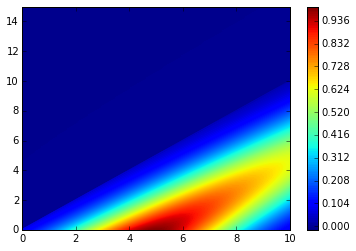
\includegraphics[width=0.5\textwidth]{_assets/advection_noPeriod.png}
    \caption{\label{diff:fig:advectionPlotNoPeriod} A simulation of the Advection Equation with a source term with in correct boundary approximations.}
  \end{figure}

% TODO: Fill in details about method
  To solve this issue, and throughout the problems here after, we imposed periodic boundary conditions on the domain so that

  \begin{equation}
    u(t, X_{\mathrm{Low}}) = u(t, X_{\mathrm{Hight}})
  \end{equation}

  for our choice of spatial domain $[X_{\mathrm{Low}}, X_{\mathrm{High}}]$. Biologically we can interpret this in terms of birth and death, as on the boundary $x = 0$ we have that the the approximation looks to the oldest individuals and the growth rate $g$ to determine the number of individuals who are born and have a weight less than the lower boundary on the domain. By taking $X_{\mathrm{low}} = k$ then we have that $u^n_{-1} = 0$ which is a suitable birth weight. When we add this condition the matrix $A$ is rewritten to include the extra term in the top right and

  \begin{equation}
    A = \begin{pmatrix}
      1 + h \cdot \mu - \lambda   & 0                         &         &                           & \lambda \\
      \lambda                     & 1 + h \cdot \mu - \lambda & 0       &\\
                                  & \lambda                   & \ddots  & \ddots                    & \\
                                  &                           & \ddots  & 1 + h \cdot \mu - \lambda & 0 \\
                                  &                           &         & \lambda                   & 1 + h \cdot \mu - \lambda
    \end{pmatrix}.
  \end{equation}

  Running a simulation for this approximation we clearly see the periodic boundary conditions.
  % TODO: Discussion of Periodic boundary conditions

  \begin{figure}
    \centering
    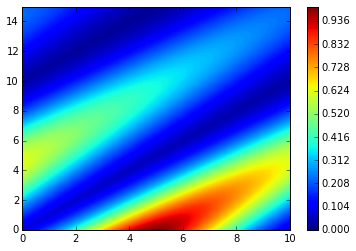
\includegraphics[width=0.5\textwidth]{_assets/advection_period.png}
    \caption{\label{diff:fig:advectionPlotPeriod} A simulation including periodic boundary conditions.}
  \end{figure}

  \section{Implicit Schemes}



\end{document}
